\section{Figuras}
\subsection{Definindo figuras}
%------------------------------------------------------------
\begin{frame}
  \frametitle{Figuras}
   Para usar figuras é necessário incluir o pacote graphicx.
   \textcolor{red}{$\backslash$usepackage\{graphicx\}}

   Este pacote suporta os seguintes formatos de figuras: \\
   \textbf{.pdf, .jpg, .jpeg, and .png}

\end{frame}


\begin{frame}[fragile]
  \frametitle{Figuras}

  A figura \ref{fig:unicentro.jpeg} ....

  \begin{minted}[fontsize=\scriptsize]{tex}
    A figura \ref{fig:unicentro.jpeg} ....

    \begin{figure}
      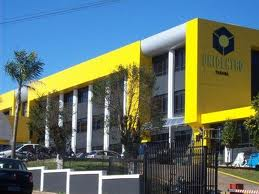
\includegraphics[scale=.5]{unicentro.jpeg}
      \label{fig:unicentro.jpeg}
      \caption{A nova Unicentro}
    \end{figure}
  \end{minted}

\end{frame}

%------------------------------------------------------------

\begin{frame}[fragile]
  \frametitle{Figuras}


    \begin{figure}
      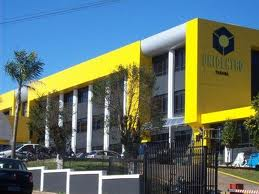
\includegraphics[scale=.5]{unicentro.jpeg}
      \label{fig:unicentro.jpeg}
      \caption{A nova Unicentro}
    \end{figure}

\end{frame}
